
\documentclass[dvipdfmx]{standalone}
\usepackage[T1]{fontenc}
\usepackage{newtxtext, newtxmath}

\usepackage{tikz}
\usetikzlibrary{trees}

\begin{document}
  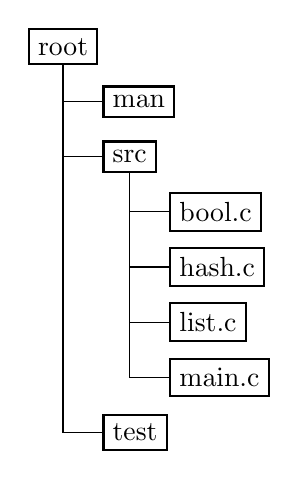
\begin{tikzpicture}[
    grow via three points={one child at (0.5,-0.7) and
    two children at (0.5,-0.7) and (0.5,-1.4)},
    edge from parent path={(\tikzparentnode.south) |- (\tikzchildnode.west)},
    every node/.style={draw=black, thick, anchor=west}
    ]
    \node {root}
      child { node {man} }
      child { node {src}
        child { node {bool.c} }
        child { node {hash.c} }
        child { node {list.c} }
        child { node {main.c} }
      }
      child [missing] {}
      child [missing] {}
      child [missing] {}
      child [missing] {}
      child { node {test} }
      ;
  \end{tikzpicture}
\end{document}
